\documentclass[a4paper, 10pt]{article}

%Paketi
\usepackage[T1]{fontenc}
\usepackage[utf8]{inputenc}
\usepackage[left=25mm, top=22mm, right=25mm, bottom=22mm, headsep=11mm]{geometry}
\usepackage{color}
\usepackage[english]{babel}
\usepackage[loadshadowlibrary, shadow]{todonotes}
\usepackage{fancyhdr}
\usepackage{setspace}
\usepackage{amsmath}
\usepackage{fix-cm}
\usepackage{colortbl}
\usepackage{multirow}
\usepackage{enumerate}
\usepackage{tikz}
\usepackage{calc}
\usepackage{ifthen}
\usepackage{pgfplots}
\usepackage{circuitikz}
\usepackage[boxed, linesnumbered, ruled]{algorithm2e}
\usepackage{hyperref}

% TikZ biblioteke
\usetikzlibrary{arrows, calc, circuits.logic.US}

%VS Code Warning Fix
\pgfplotsset{compat=1.18}

%Boje
\definecolor{lavander}{RGB}{230, 230, 250}
\definecolor{redBrick}{RGB}{194, 42, 20}
\definecolor{orange}{RGB}{255, 128, 0}
\definecolor{cbGray}{RGB}{145, 145, 145}
\definecolor{tikZSivaText}{RGB}{77, 77, 77}
\definecolor{tikZSivaCrtanje}{RGB}{128, 128, 128}
\definecolor{magenta}{RGB}{237, 2, 140}
\definecolor{lightBlue}{RGB}{0, 174, 239}
\definecolor{bronze}{RGB}{191, 128, 64}
\definecolor{urlColor}{RGB}{0, 174, 239}
\definecolor{lightPurple}{RGB}{200, 193, 229}
\definecolor{borderColor}{RGB}{132, 129, 125}
\definecolor{lightYellow}{RGB}{255, 255, 209}
\definecolor{lightBlue}{RGB}{169, 197, 219}
\definecolor{lightGreen}{RGB}{147, 188, 109}
\definecolor{darkBlue}{RGB}{74, 54, 173}
\definecolor{darkGreen}{RGB}{80, 118, 38}
\definecolor{basSvijetlaSvijetlaSiva}{RGB}{253, 253, 253}
\definecolor{basSvijetlaTamnaSiva}{RGB}{236, 236, 236}


%Brojači
\newcounter{brojacTabela}
\newcounter{brojacSlika}

%Nove komande
\newcommand{\boldItalicColored}[2]{\color{#1}\textbf{\textsl{#2}}\color{black}}
\newcommand{\commandNameText}[1]{\texttt{\color{redBrick}\textbackslash#1\color{black}\{\}}}
\newcommand{\typewriterColored}[2]{\color{#1}\texttt{#2}\color{black}}
\newcommand{\tableAlpha}[1]{$#1 \cdot 10^{-4}$}
\newcommand{\nazivTabele}[1]
{
    \vspace{2mm}
    \vspace{1.5mm}
    \stepcounter{brojacTabela}
    \hypertarget{Tabelica: \arabic{brojacTabela}}{Tabelica} \arabic{brojacTabela}: #1
    \addcontentsline{lot}{table}{\arabic{brojacTabela} \hspace{4mm} #1}
}
\newcommand{\nazivSlike}[1]
{
    \vspace{2mm}
    \vspace{1.5mm}
    \stepcounter{brojacSlika}
    \hypertarget{Sličica: \arabic{brojacSlika}}{Sličica} \arabic{brojacSlika}: #1
    \addcontentsline{lof}{figure}{\arabic{brojacSlika} \hspace{4mm} #1}
}

%Linkovi
\hypersetup{
    colorlinks,
    allcolors = black,
    urlcolor = urlColor
}

%Stilovi
\fancypagestyle{prvaStranica}{
    \lhead{} \chead{} \rhead{}
    \lfoot{} \cfoot{\thepage} \rfoot{}
    \renewcommand{\headrulewidth}{0pt}
}

\fancypagestyle{tptp_style}{
    \lhead{\textsc{Bjelić Elnur}} \chead{} \rhead{
\includegraphics[scale=0.06, trim=0.25mm 0.25mm 0.25mm 0.25mm]{./logo.pdf}}
    \renewcommand{\headrulewidth}{0.23pt}    
}

\pagestyle{tptp_style}
\begin{document}
    %Promjenjene komande
    \renewcommand{\contentsname}{Doista kratak sadržaj}
    \renewcommand{\listtablename}{Mala lista tabela}
    \renewcommand{\listfigurename}{Popis slika}

    \thispagestyle{prvaStranica}

    \noindent Univerzitet u Tuzli \hfill{\textsc{Proljeće 2023.}} \newline{}
    Fakultet elektrotehnike \hfill{Bjelić Elnur} \newline{}
    TK001 \newline{}
    \begin{center}
        \vspace{5mm}
        \begin{spacing}{1}
            \hspace{18pt}\LARGE{\textsc{Tehnologije za Podršku Tehničkom Pisanju}} \newline{}
            \LARGE{\textsc{Zadaća I  \todo[backgroundcolor=lavander, linecolor=lavander]{\scriptsize{Naslov dokumenta vertikalno je pomjeren za 5 mm u odnosu na prethodni i naredni sadržaj.}}}}
        \end{spacing}
        \vspace{5mm}
        \begin{abstract}
            \boldItalicColored{black}{Prije svega }ovu zadaću ćete uraditi \boldItalicColored{redBrick}{sami bez varanja}, \boldItalicColored{black}{umjetne inteligencije i botova sa Interneta}. U okviru zadaće pokušat ćete domonstrirati svo stečeno znanje iz predmeta \textit{Tehnologije za podršku tehničkom pisanju} vezano za \LaTeX. Pažljivo analizirati dokument i replicirati sadržaj istog (stranice od 1 do 6). Obratiti pažnju na detalje u originalnom dokumentu te koristit pravila i principe \LaTeX-a za repliciranje istog. Vaš dokument mora biti \underline{vjerodostojna kopija} originalnom dokumentu (osim dijela prezime i ime, i broj indeksa). Kao rezultat, studenti će \boldItalicColored{orange}{predati kod } (*.tex i *.pdf file).
        \end{abstract}
    \end{center}
    \tableofcontents
    \listoffigures
    \listoftables
    \section{Stil dokumenta}
    Uslijed nedostatka podrške za govorno područje \textit{Bosne i Hercegovine} u paketu \texttt{babel}, potrebno je redefinirati funkcionalnost komande \commandNameText{contentsname} promijeniti naziv liste sadržaja u \textit{Doista kratak sadržaj}. Na sličan način ponoviti za komande \commandNameText{listfigurename}, \commandNameText{listtablename}, \commandNameText{figurename} i \commandNameText{tablename}
    \subsection{Margine dokumenta}
    Margine stranica dokumenta su postavljene na sljedeći način: lijeva: 25 mm, donja: 22 mm, gornja: 22 mm i desna: 25 mm. Da bi smo znali da je ovo vaša zadaća, na mjesto \textit{Prezime Ime} upisat vaše \underline{ime i prezime}. Dobro \boldItalicColored{redBrick}{obratiti }pažnju da se na tekućoj i narednim stranicama dokumenta zadaće, nalazi zaglavlje i podnožje a na prethodnoj ne! U okviru zadaće kreirati \LaTeX\ komande i okruženja gdje god to ima smisla.
    \subsection{Zaglavlje i podnožje dokumenta}
    Stil dokumenta generirati sa komandama iz paketa \underline{fancyhdr} pri čemu će se novi stil zvati \texttt{tptp\_style}. Slika unutar zaglavlja stranice dokumenta (\textit{logo.pdf}) je \texttt{hipotetički }logo fakulteta a skaliran je na 0.06 te je prostor oko slike skraćen je za 0.25 mm sa svih strana .\todo[backgroundcolor=lavander, linecolor=lavander]{\scriptsize{Dogovorili smo se da \boldItalicColored{redBrick}{nema }varanja!}} Debljina linije u zaglavlju je 0.23 pt.
    \section{Matematički mod i tabele}
    \subsection{Matematički mod}
    U \LaTeX-u smo upoznali matematički mod\footnote{Ne zaboravite da matematički mod zahtjeva uključenje paketa \texttt{amsmath}.} koji nam omogućava i formatiranje matrica \newline{}
    \begin{displaymath}
        \left[
            \begin{matrix}
                \vspace{2mm}
                3 & 4 & 2 \\
                5 & 0 & 2
            \end{matrix}
        \right]
        \left[
            \begin{matrix}
                \vspace{2mm}
                1 & 2 & 3 \\
                \vspace{2mm}
                3 & 0 & 1 \\
                0 & 2 & 1
            \end{matrix}
        \right]
        =
        \left[
            \begin{matrix}
                \vspace{2mm}
                15 & 10 & 15 \\
                5 & 14 & 17
            \end{matrix}
        \right]
    \end{displaymath}
    U sljedećem primjeru imamo jednu složenu matematičku formulu za izračun Bassel-ovih koeficijenata prve vrste
    \begin{equation}
        J_{\alpha}(x) = \sum_{m=0}^{\infty}\frac{(-1)^m}{m!\ \Gamma(m + \alpha + 1)}\left(\frac{x}{2}\right)^{2m + \alpha}
    \end{equation}
    U toku prvog semestra upoznali ste se sa Amper-ovim zakonom koji je definiran na sljedeći način
    \begin{equation}
        \oint_C \textbf{B} \cdot \text{d}\boldsymbol{\ell} = \mu_0 \iint_S \textbf{J} \cdot \text{d}\textbf{S} = \mu_0I_{\text{enc}}
    \end{equation}
    U izrazu 3 imamo dat proračun uslovne vjerovatnoće $p(y_k|c_k)$ simbola $y_k$ ako je poslat simbol $c_k$, turbo konvolucionog dekodera:
    \begin{equation}
        p(y_k|c_k) = \prod_{i,j}p(y_k^{i,j}|c_k^{i,j}) = \prod_{i,j}\frac{1}{\sqrt{2\pi}\sigma}\text{exp}\left(-\frac{1}{2\sigma^2}\left(y_k^{i,j}-c_k^{i,j}\right)^2\right)
    \end{equation}
    U sljedećem redu ispisan je tekst sa fontom \textit{Palantino-Roman (ppl)} visine \textit{60 pt}\footnote{Obratiti pažnju da će nam trebati paket \texttt{fix-cm}} \newline{}
    \begin{center}
        {\fontfamily{ppl}\selectfont\fontsize{60pt}{1pt}\selectfont{ONLY HUMAN}}
    \end{center}
    \subsection{Tabele}
    U nastavku imamo dvije tabele postavljene koristeći okruženja \typewriterColored{blue}{minipage}, \typewriterColored{blue}{tabular }i \typewriterColored{blue}{table}. Ta tabele je redefinirana funkcionalnost komande \commandNameText{arraystretch} na vrijednost 1.1 \newline{}
    \begin{minipage}{.7\textwidth}
            \centering
            \renewcommand{\arraystretch}{1.1}
            \begin{tabular}{c c c c c}
                \hline \hline
                \rowcolor[RGB]{77, 77, 77}\multicolumn{2}{c}{\color{white}\textbf{Poluprovodnik}} & \color{white}$E_{g0}\ (eV)$ & \color{white}$\alpha\ (eV/K)$ & \color{white}$\beta\ (K)$\\
                \hline \hline
                \rowcolor[RGB]{242, 242, 242}Si & Silicij & 1.17 & \tableAlpha{4.73} & 636\\
                Ge & Germanijum & 0.74 & \tableAlpha{4.77} & 235\\
                \rowcolor[RGB]{242, 242, 242}GaAs & Galijum Arsenid & 1.52 & \tableAlpha{5.41} & 204\\
                AlAs & Aluminijum Sulfid & 2.42 & \tableAlpha{6.00} & 408\\
                \rowcolor[RGB]{242, 242, 242}InAs & Indijum Arsenid & 0.42 & \tableAlpha{2.50} & 75\\
                InP & Indijum Fostat & 1.42 & \tableAlpha{3.63} & 162\\
                \rowcolor[RGB]{242, 242, 242}GaP & Galijum Fosfat & 2.33 & \tableAlpha{5.77} & 372\\
                \hline \hline
            \end{tabular}
            \nazivTabele{Parametri modela širine zabranjenog pojasa}
    \end{minipage}
    \begin{minipage}{.3\textwidth}
        \renewcommand{\arraystretch}{1.4}
        \centering
        \begin{tabular}{| l | c | r |}
            \hline \hline
            \multirow{2}{*}{MR2} & \multicolumn{2}{c|}{MC2} \\
            \cline{2-2}
            & D & \cellcolor[RGB]{255, 230, 204}E \\
            \hline
            \cellcolor[RGB]{255, 251, 214}M & A & N \\
            \hline
            \multicolumn{2}{|c|}{\cellcolor[RGB]{204, 204, 255}MC1} & \multirow{2}{*}{MR1} \\
            \cline{1-2}
            A & B & \\
            \hline
            C & \cellcolor[RGB]{250, 213, 229}T & Y \\
            \hline \hline \hline
        \end{tabular}
        \nazivTabele{Spajanje ćelija}
    \end{minipage}
    \begin{center}
        \fbox{\colorbox{cbGray}{\parbox{133mm}{
            U malom ograničenom paragrafu širine 133 mm prikazana je lista mali Grčkih karaktera, velikih Rimskih cifara\footnote{} i heksadecimalnih cifara\footnote{}
            \color{white}
            \begin{enumerate}[a)]
                \item \scriptsize{\texttt{0, 1, 2, 3, 4, 5, 6, 7, 8, 9, A, B, C, D, E i F}}
                \item $I$, $V$, $X$, $L$, $D$, $C$ i $M$,
                \item \small{}$\alpha, ~\Delta, ~\sigma, ~\Gamma, ~\rho, ~\Psi, ~\mu, ~\gamma, ~\epsilon, ~\Omega, ~\psi, ~\pi, ~\kappa, ~\vartheta, ~\delta, ~\omega, ~\lambda, ~\tau.$ 
            \end{enumerate}
        }}}
    \end{center}
    \section{Paketi za crtanje u \LaTeX-u}
    \subsection{TikZ paket}
    Na slikama \hyperref[slika1]{1} i \hyperref[slika2]{2} prikazani su konstalacijski dijagrami QPSK i 16QAM modulacijskih tehnika u signalnom prostoru. Slike su postavljene jedna pored druge koristeći dva okruženja \texttt{minipage}\footnote{Neki od korisnih atributa za ktikz su: stealth', dashed, fill, color, draw, opacity. Za implementaciju koristiti petlju \boldItalicColored{redBrick}{foreach}.}. \newline{} \newline{}
    \begin{minipage}{0.5\textwidth}
        \centering
        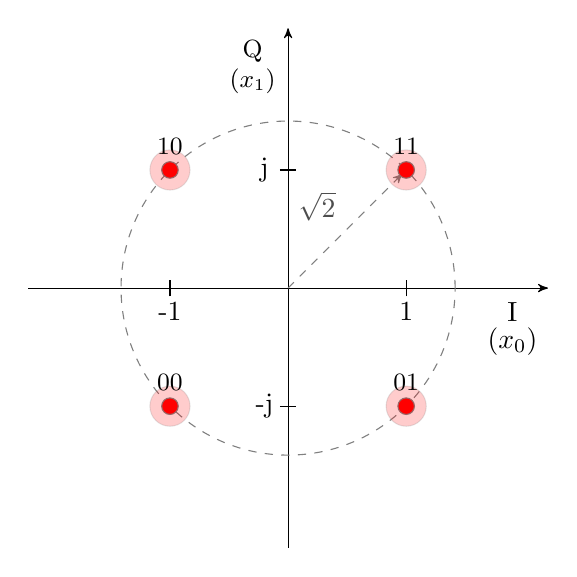
\begin{tikzpicture}[scale=1.5]
            \draw[->, >=stealth'] (0, -2.2)--(0, 2.2);
            \draw (-0.3, 2) node[] {\small{Q}};
            \draw (-0.3, 1.75) node[] {\small{($x_1$)}};
            \draw[->, >=stealth'] (-2.2, 0)--(2.2, 0);
            \draw (1.9, -0.2) node[] {I};
            \draw (1.9, -0.45) node[] {($x_0$)};
            \draw (1, -0.07)--(1, 0.07);
            \draw (1, -0.2) node[] {1};
            \draw (-1, -0.07)--(-1, 0.07);
            \draw (-1, -0.2) node[] {-1};
            \draw (-0.07, 1)--(0.07, 1);
            \draw (-0.2, 1) node[] {j};
            \draw (-0.07, -1)--(0.07, -1);
            \draw (-0.2, -1) node[] {-j};
            \draw[color=tikZSivaCrtanje, dashed] (0, 0) circle(1.41421);
            \draw[->, >=stealth', color=tikZSivaCrtanje, dashed] (0, 0)--(0.97, 0.97) node[midway, above left] {\color{tikZSivaText}$\sqrt{2}$\color{black}};
            \foreach \x in {-1, 1} {
                \foreach \y in {1, -1} {
                    \draw[color=tikZSivaCrtanje, fill=red] (\x, \y) circle(0.07);
                    \draw[color=tikZSivaCrtanje, fill=red, opacity=0.2] (\x, \y) circle(0.17);
                    \draw (\x, \y + 0.2) node[] {\color{black}\small{\ifthenelse{\y < 0}{0}{1}\ifthenelse{\x < 0}{0}{1}}};
                }
            }
        \end{tikzpicture} \newline{}
        \nazivSlike{Konstalacijski dijagram QPSK}
        \label{slika1}
    \end{minipage}
    \begin{minipage}{0.5\textwidth}
        \centering
        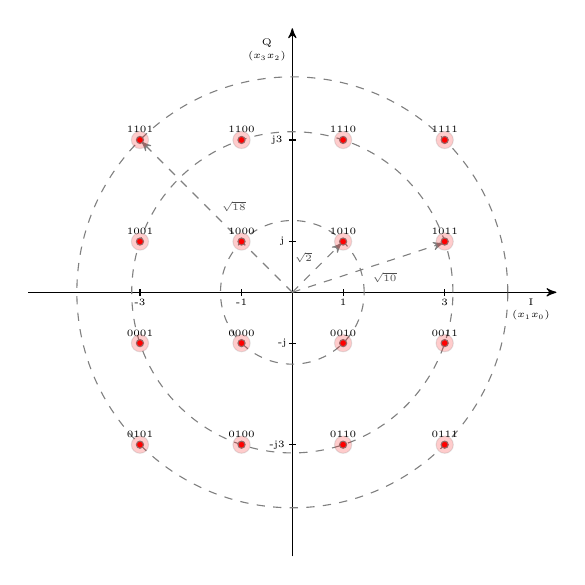
\begin{tikzpicture}[scale=0.645]
            \fontsize{3.5pt}{1pt}
            \draw[->, >=stealth'] (0, -5.2)--(0, 5.2);
            \draw (-0.5, 4.9) node[] {Q};
            \draw (-0.5, 4.65) node[] {($x_3x_2$)};
            \draw[->, >=stealth'] (-5.2, 0)--(5.2, 0);
            \draw (4.7, -0.2) node[] {I};
            \draw (4.7, -0.45) node[] {($x_1x_0$)};
            \draw (1, -0.07)--(1, 0.07);
            \draw (1, -0.2) node[] {1};
            \draw (-1, -0.07)--(-1, 0.07);
            \draw (-1, -0.2) node[] {-1};
            \draw (-0.07, 1)--(0.07, 1);
            \draw (-0.2, 1) node[] {j};
            \draw (-0.07, -1)--(0.07, -1);
            \draw (-0.2, -1) node[] {-j};
            \draw (3, -0.07)--(3, 0.07);
            \draw (3, -0.2) node[] {3};
            \draw (-3, -0.07)--(-3, 0.07);
            \draw (-3, -0.2) node[] {-3};
            \draw (-0.07, 3)--(0.07, 3);
            \draw (-0.3, 3) node[] {j3};
            \draw (-0.07, -3)--(0.07, -3);
            \draw (-0.3, -3) node[] {-j3};
            \draw[color=tikZSivaCrtanje, dashed] (0, 0) circle(1.41421);
            \draw[->, >=stealth', color=tikZSivaCrtanje, dashed] (0, 0)--(0.97, 0.97) node[midway, above left] {\color{tikZSivaText}$\sqrt{2}$\color{black}};
            \draw[color=tikZSivaCrtanje, dashed] (0, 0) circle(3.16227);
            \draw[->, >=stealth', color=tikZSivaCrtanje, dashed] (0, 0)--(2.97, 0.97) node[midway, below right] {\color{tikZSivaText}$\sqrt{10}$\color{black}};
            \draw[color=tikZSivaCrtanje, dashed] (0, 0) circle(4.24264);
            \draw[->, >=stealth', color=tikZSivaCrtanje, dashed] (0, 0)--(-2.97, 2.97) node[midway, above right] {\color{tikZSivaText}$\sqrt{18}$\color{black}};
            \foreach \x in {-3, -1, 1, 3} {
                \foreach \y in {3, 1, -1, -3} {
                    \draw[color=tikZSivaCrtanje, fill=red] (\x, \y) circle(0.07);
                    \draw[color=tikZSivaCrtanje, fill=red, opacity=0.2] (\x, \y) circle(0.17);
                    \draw (\x, \y + 0.2) node[] {\color{black}\fontsize{3.5pt}{1pt}{\ifthenelse{\y > 0}{1}{0}\ifthenelse{\y = 3 \OR{} \y = -3}{1}{0}\ifthenelse{\x > 0}{1}{0}\ifthenelse{\x = 3 \OR{} \x = -3}{1}{0}}};
                }
            }
        \end{tikzpicture} \newline{}
        \nazivSlike{Konstalacijski dijagram 16QAM}
        \label{slika2}
    \end{minipage}
    Talasni oblik pobude i izlaz RS-FF prikazan je na slici \hyperref[slika3]{3}. Debljina linije krive je 1.5 pt a opseg apscise je od -0.25 do 9.5 dok je ordinate od -0.25 do 1.5. \newline{}
    \newpage
    \begin{figure}[t]
        \centering
        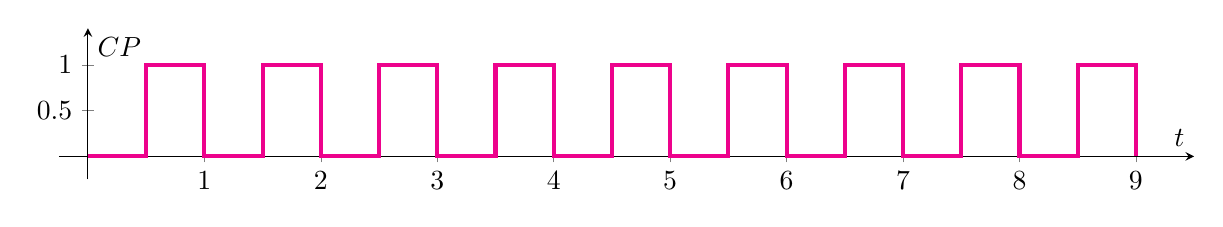
\begin{tikzpicture}
            \begin{axis}[
                width = 16cm,
                height = 3.5cm,
                axis y line=middle,
                axis x line=middle,
                xtick = {1, 2, 3,..., 9},
                ytick = {0.5, 1},
                xmin = -0.25,
                xmax = 9.5,
                ymin = -0.25,
                ymax = 1.4,
                xlabel = {$t$},
                ylabel = {$CP$},
            ]
                \addplot+[magenta, line width = 1.5pt, mark = none, const plot]
                coordinates{
                    (0, 0) (0.5, 0) (0.5, 1)
                    (1, 1) (1, 0) (1.5, 0)
                    (1.5, 1) (2, 1) (2, 0)
                    (2.5, 0) (2.5, 1) (3, 1)
                    (3, 0) (3.5, 0) (3.5, 1)
                    (4, 1) (4, 0) (4.5, 0)
                    (4.5, 1) (5, 1) (5, 0)
                    (5.5, 0) (5.5, 1) (6, 1)
                    (6, 0) (6.5, 0) (6.5, 1)
                    (7, 1) (7, 0) (7.5, 0)
                    (7.5, 1) (8, 1) (8, 0)
                    (8.5, 0) (8.5, 1) (9, 1)
                    (9, 0)
                };
            \end{axis}
        \end{tikzpicture}
        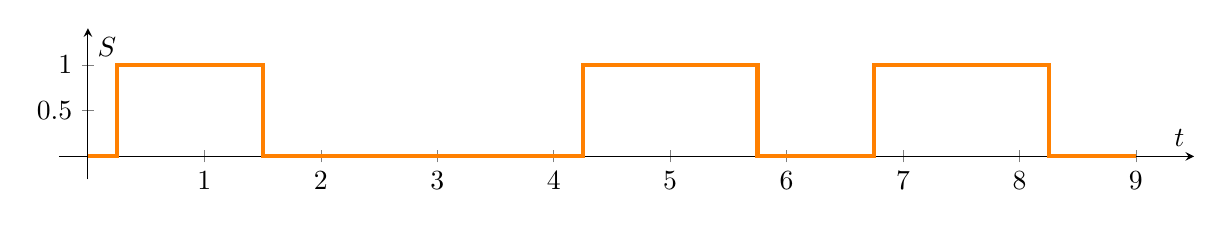
\begin{tikzpicture}
            \begin{axis}[
                width = 16cm,
                height = 3.5cm,
                axis y line=middle,
                axis x line=middle,
                xtick = {1, 2, 3,..., 9},
                ytick = {0.5, 1},
                xmin = -0.25,
                xmax = 9.5,
                ymin = -0.25,
                ymax = 1.4,
                xlabel = {$t$},
                ylabel = {$S$},
            ]
                \addplot+[orange, line width = 1.5pt, mark = none, const plot]
                coordinates{
                    (0, 0) (0.25, 0) (0.25, 1)
                    (1.5, 1) (1.5, 0) (4.25, 0)
                    (4.25, 1) (5.75, 1) (5.75, 0)
                    (6.75, 0) (6.75, 1) (8.25, 1)
                    (8.25, 0) (9, 0)
                };
            \end{axis}
        \end{tikzpicture}
        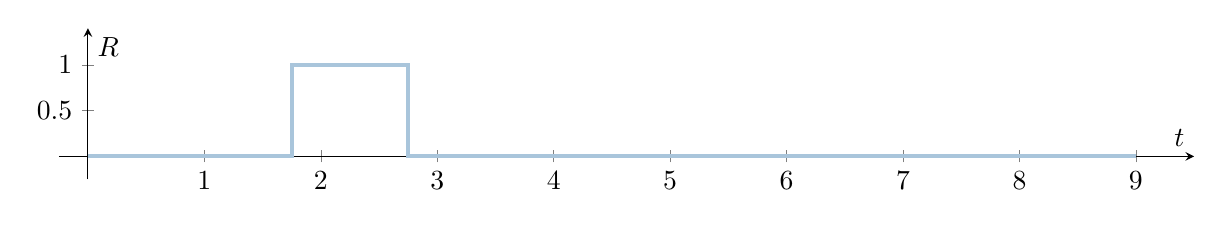
\begin{tikzpicture}
            \begin{axis}[
                width = 16cm,
                height = 3.5cm,
                axis y line=middle,
                axis x line=middle,
                xtick = {1, 2, 3,..., 9},
                ytick = {0.5, 1},
                xmin = -0.25,
                xmax = 9.5,
                ymin = -0.25,
                ymax = 1.4,
                xlabel = {$t$},
                ylabel = {$R$},
            ]
                \addplot+[lightBlue, line width = 1.5pt, mark = none, const plot]
                coordinates{
                    (0, 0) (1.75, 0) (1.75, 1)
                    (2.75, 1) (2.75, 0) (9, 0)
                };
            \end{axis}
        \end{tikzpicture}
        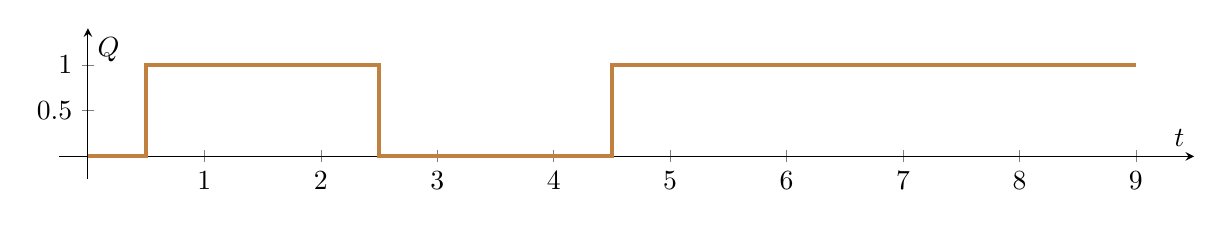
\begin{tikzpicture}
            \begin{axis}[
                width = 16cm,
                height = 3.5cm,
                axis y line=middle,
                axis x line=middle,
                xtick = {1, 2, 3,..., 9},
                ytick = {0.5, 1},
                xmin = -0.25,
                xmax = 9.5,
                ymin = -0.25,
                ymax = 1.4,
                xlabel = {$t$},
                ylabel = {$Q$},
            ]
                \addplot+[bronze, line width = 1.5pt, mark = none, const plot]
                coordinates{
                    (0, 0) (0.5, 0) (0.5, 1)
                    (2.5, 1) (2.5, 0) (4.5, 0)
                    (4.5, 1) (9, 1)
                };
            \end{axis}
        \end{tikzpicture}\\
        \nazivSlike{Talasni oblik signala na izlazi SR bistabila}
        \label{slika3}
    \end{figure}
    \subsection{Električne, blok sheme i \boldItalicColored{redBrick}{circuitikz }paket}
    Na slici \hyperref[slika4]{4} prikazana je implementacija logičke funkcije \textit{f} sa NOR logičkim kolima metodom supstitucije\footnote{Prilikom crtanja logičke sheme neophodno je uključiti \textsl{tikz} biblioteku \textsl{circuits.logic.US}}. Ukoliko imate poteškoća sa realizacijom logičke i električne sheme, možete se poslužiti primjerima iz kratkog \textsl{manuala} \texttt{circuitikz }paketa, koje se nalazi na CTAN \href{http://texdoc.net/show.php?pkg=circuitikz}{stranici}.
    \begin{figure}[h]
        \centering
        \begin{circuitikz}
            \scriptsize{}
            \ctikzset{logic ports=ieee}
            \draw (0, 0) node[above] {A} -- (0, -7.3);
            \draw (0.6, 0) node[above] {B} -- (0.6, -7.3);
            \draw (1.2, 0) node[above] {C} -- (1.2, -7.3);
            \draw (2.2, -1) node[nor port, number inputs = 3, scale = 0.4] (norKolo1) {};
            \draw (0, -0.85) to[short, *-] (norKolo1.in 1);
            \draw (0.6, -1) to[short, *-] (norKolo1.in 2);
            \draw (1.2, -1.145) to[short, *-] (norKolo1.in 3);
            \draw (2.2, -2.5) node[nor port, scale = 0.35] (norKolo2) {};
            \draw (0.6, -2.5) to[short, *-*] (1.7, -2.5);
            \draw (1.7, -2.5) |- (norKolo2.in 1);
            \draw (1.7, -2.5) |- (norKolo2.in 2);
            \draw (2.2, -3.7) node[nor port, scale = 0.35] (norKolo3) {};
            \draw (0, -3.7) to[short, *-*] (1.7, -3.7);
            \draw (1.7, -3.7) |- (norKolo3.in 1);
            \draw (1.7, -3.7) |- (norKolo3.in 2);
            \draw (2.2, -5.2) node[nor port, scale = 0.35] (norKolo4) {};
            \draw (1.2, -5.2) to[short, *-*] (1.7, -5.2);
            \draw (1.7, -5.2) |- (norKolo4.in 1);
            \draw (1.7, -5.2) |- (norKolo4.in 2);
            \draw (2.2, -6.7) node[nor port, scale = 0.35] (norKolo5) {};
            \draw (1.2, -6.7) to[short, *-*] (1.7, -6.7);
            \draw (1.7, -6.7) |- (norKolo5.in 1);
            \draw (1.7, -6.7) |- (norKolo5.in 2);
            \draw (2.5, -4.3) node[nor port, scale = 0.35] (norKolo6) {};
            \draw (0.6, -4.3) to[short, *-*] (2, -4.3);
            \draw (2, -4.3) |- (norKolo6.in 1);
            \draw (2, -4.3) |- (norKolo6.in 2);
            \draw (2.5, -5.8) node[nor port, scale = 0.35] (norKolo7) {};
            \draw (0, -5.8) to[short, *-*] (2, -5.8);
            \draw (2, -5.8) |- (norKolo7.in 1);
            \draw (2, -5.8) |- (norKolo7.in 2);
            \draw (3.4, -1.9) node[nor port, number inputs = 3, scale = 0.4] (norKolo8) {};
            \draw (0, -1.75) to[short, *-] (norKolo8.in 1);
            \draw (1.2, -1.9) to[short, *-] (norKolo8.in 2);
            \draw (norKolo2.out) |- (2.73, -2.5) |- (norKolo8.in 3);
            \draw (3.4, -3.1) node[nor port, number inputs = 3, scale = 0.4] (norKolo9) {};
            \draw (0.6, -2.95) to[short, *-] (norKolo9.in 1);
            \draw (1.2, -3.1) to[short, *-] (norKolo9.in 2);
            \draw (norKolo3.out) |- (2.73, -3.7) |- (norKolo9.in 3);
            \draw (3.4, -4.6) node[nor port, number inputs = 3, scale = 0.4] (norKolo10) {};
            \draw (norKolo6.out) |- (2.92, -4.3) |- (norKolo10.in 1);
            \draw (0, -4.6) to[short, *-] (norKolo10.in 2);
            \draw (norKolo4.out) |- (2.785, -5.2) |- (norKolo10.in 3);
            \draw (3.4, -6.1) node[nor port, number inputs = 3, scale = 0.4] (norKolo11) {};
            \draw (norKolo7.out) |- (2.92, -5.8) |- (norKolo11.in 1);
            \draw (0.6, -6.1) to[short, *-] (norKolo11.in 2);
            \draw (norKolo5.out) |- (2.785, -6.7) |- (norKolo11.in 3);
            \draw (5.5, -1.3) node[nor port, number inputs = 5, scale = 0.55] (norKolo12) {};
            \draw (norKolo1.out) |- (2.85, -1) |- (norKolo12.in 1);
            \draw (norKolo8.out) |- (3.9, -1.9) |- (norKolo12.in 2);
            \draw (norKolo9.out) |- (4.05, -3.1) |- (norKolo12.in 3);
            \draw (norKolo10.out) |- (4.2, -4.6) |- (norKolo12.in 4);
            \draw (norKolo11.out) |- (4.35, -6.1) |- (norKolo12.in 5);
            \draw (norKolo12.out) |- (6.3, -1.3) node[right, above] {$f$};
        \end{circuitikz}\\
        \nazivSlike{Implementacija logičke funkcije $f$ sa NOR logičkim kolima}
        \label{slika4}
    \end{figure}\\
    Na slici \hyperref[slika5]{5} prikazana je ekvivalentna shema jednog hipotetičkog pojačavačkog stepena. \todo[backgroundcolor=lavander, linecolor=lavander]{\scriptsize{Upotrijebiti opciju \texttt{american} u okruženju \typewriterColored{blue}{circuitikz }za generiranje simbola prema američkom standardu označavanja elektroničkih komponenti.}}U okviru električne sheme (na slici \hyperref[slika5]{5}) korištene su sljedeće komponente: \texttt{R}, \texttt{L}, \texttt{C} i \texttt{american current source}.
    \pagebreak
    \begin{figure}[ht]
        \centering
        \begin{circuitikz}[american]
            \draw (0, 0) to[short, i_ = $i_{ul}$, o-*] (2, 0) node[above] {$\text{A}_1$};
            \draw (2, -5.4) to[short, color = green, L, l = $L_2$, i = $i_5$] (4.7, -5.4) {};
            \draw (10.05, -5.4) -- (7.1, -5.4) {};
            \draw (4.7, -5.4) to[short, color = tikZSivaCrtanje, R, l = $R_6$, i = $i_6$] (8.3, -5.4) {};
            \draw (7.6, 0) to[short, color = red, L, l_ = $L_1$, i =$i_4$, *-*] (7.6, -2.7) {};
            \draw (4.7, -2.7) to[short, color = tikZSivaCrtanje, R, l = $R_5$, i = $i_6$, *-*] (4.7, -5.4) {};
            \draw (2, 0) to[short, L, l_ = $L_5$, i = $i_2$, -*] (4.7, 0) node[above] {$\text{B}_1$};
            \draw (7.6, 0) to[short, color = bronze, I, l = $gi_1$] (4.7, 0) {};
            \draw (7.6, 0) -- (8.1, 0) node[above] {$D_1$};
            \draw (8.1, 0) to[short, R, l_ = $R_C$, i = $i_C$, -*] (10.9, 0) node[above] {$\text{E}_1$};
            \draw (10.9, 0) -- (12.7, 0) {};
            \draw (12.7, 0) to[short, i_ = $i_{iz}$] (14.1, 0) {};
            \draw (2, 0) to[short, C, l = $C_1$, i = $i_1$, -*] (2, -2.7) {};
            \draw (4.7, 0) to[short, C, l_ = $C_{E1}$, i = $i_{e1}$] (4.7, -2.7) {};
            \draw (10.9, -2.7) node[below] {$\text{F}_1$} to[short, color = magenta, I, l = $hi_2$] (10.9, 0) {};
            \draw (12.7, 0) to[short, R, l_ = $Z_{E2}$] (12.7, -2.7) {};
            \draw (14.1, 0) to[short, color = blue, R, l_ = $R_p$] (14.1, -2.7) {};
            \draw (0, -2.7) to[short, o-] (14.1, -2.7) {};
            \draw (2, -2.7) to[short, R, l = $R_g$, i = $i_g$] (2, -5.4) {};
            \draw (10.05, -2.7) to[short, *-] (10.05, -5.4) {};
            \scriptsize{}
            \draw (0,-0.65) node[above]{+};
            \draw (0,-1.35) node{$u_{ul}$};
            \draw (0,-2.1) node[below]{-};
            \draw (8.4,-0.65) node[above]{+};
            \draw (8.4,-1.35) node{$u_{12}$};
            \draw (8.4,-2.1) node[below]{-};
            \draw (14.9,-0.65) node[above]{+};
            \draw (14.9,-1.35) node{$u_{iz}$};
            \draw (14.9,-2.1) node[below]{-};
            \draw[->, >=latex', rounded corners = 5pt, color = red] (0.5, -1.35) -- (0.5, -0.46) -- (4.2, -0.46) -- (4.2, -2.25) -- (0.5, -2.25);
            \draw[->, >=latex', rounded corners = 5pt, color = blue, dashed] (8.7, -1.35) -- (8.7, -0.46) -- (13.2, -0.46) -- (13.2, -2.25) -- (8.7, -2.25);
        \end{circuitikz}\\
        \nazivSlike{Ekvivalentna shema hipotetičkog pojačavača}
        \label{slika5}
    \end{figure}
    Slika \hyperref[slika6]{6} predstavlja model OFDM modulatora. Prilikom crtanja modela i ostalih \texttt{tikz} baziranih dijagrama/grafika/slika možete se poslužiti aplikacijama kao što je \textsl{ktikz}, \textsl{QTikZ}, \textsl{TpX} i sl.
    \begin{figure}[h!]
        \centering
        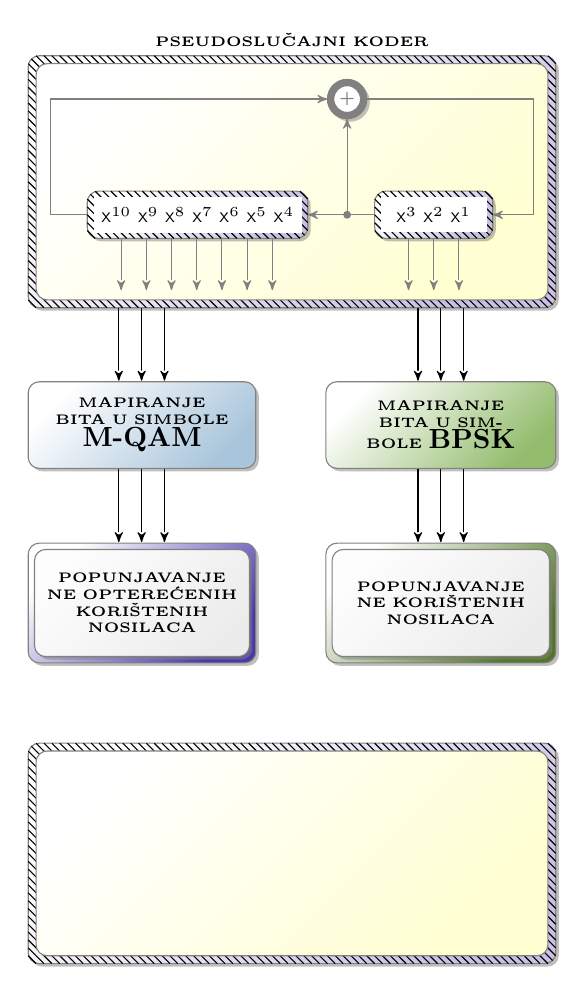
\begin{tikzpicture}
            \tiny{}
            \draw[borderColor, right color = white, left color = lightPurple, rounded corners, shading angle = 225, anchor = south, drop shadow] (0, 0) rectangle (6.7, -3.2);
            \foreach \x in {0, 0.1, 0.2,..., 6.6} {
                \foreach \y in {-3.1, -3.0,..., 0.1} {
                    \pgfmathparse{abs(\x) < 0.001 ? int(0) : int(1)}
                    \ifthenelse{\pgfmathresult = 0}
                    {
                        \pgfmathparse{abs(\y) < 0.001 ? int(0) : int(1)}
                        \ifthenelse{\pgfmathresult = 0}
                        {
                            \draw (\x + 0.04, \y - 0.04) -- (\x + 0.1, \y - 0.1);
                        }
                        {
                            \draw (\x, \y) -- (\x + 0.1, \y - 0.1);
                        }
                    }
                    {
                        \pgfmathparse{abs(6.7 - (\x + 0.1)) < 0.001 ? int(0) : int(1)}
                            \ifthenelse{\pgfmathresult = 0}
                            {
                                \pgfmathparse{abs(3.2 + (\y - 0.1)) < 0.001 ? int(0) : int(1)}
                                \ifthenelse{\pgfmathresult = 0}
                                {
                                    \draw (\x, \y) -- (\x + 0.06, \y - 0.06);
                                }
                                {
                                    \draw (\x, \y) -- (\x + 0.1, \y - 0.1);
                                }
                            }
                            {
                                \draw (\x, \y) -- (\x + 0.1, \y - 0.1);
                            }
                    }
                    \pgfmathparse{abs(\x - 6.7) < 0.001 ? int(0) : int(1)}
                    \ifthenelse{\pgfmathresult = 0}
                }
            }
            \draw[borderColor, right color = white, left color = lightYellow, rounded corners, shading angle = 225, anchor = south] (0.1, -0.1) rectangle (6.6, -3.1);
            \draw[tikZSivaCrtanje, fill = tikZSivaCrtanje, drop shadow] (4.05, -0.55) circle(0.25);
            \draw[tikZSivaCrtanje, fill = white] (4.05, -0.55) circle(0.17) node[] {\textbf{+}};
            \draw[borderColor, right color = white, left color = lightPurple, rounded corners, shading angle = 225, anchor = south, drop shadow] (0.75, -1.72) rectangle (3.55, -2.32);
            \foreach \x in {0.75, 0.85,..., 3.55} {
                \foreach \y in {-2.22, -2.12,..., -1.62} {
                    \pgfmathparse{abs(\x - 0.75) < 0.001 ? int(0) : int(1)}
                    \ifthenelse{\pgfmathresult = 0}
                    {
                        \pgfmathparse{abs(\y + 1.72) < 0.001 ? int(0) : int(1)}
                        \ifthenelse{\pgfmathresult = 0}
                        {
                            \draw (\x + 0.04, \y - 0.04) -- (\x + 0.1, \y - 0.1);
                        }
                        {
                            \draw (\x, \y) -- (\x + 0.1, \y - 0.1);
                        }
                    }
                    {
                        \pgfmathparse{abs(3.55 - (\x + 0.1)) < 0.001 ? int(0) : int(1)}
                            \ifthenelse{\pgfmathresult = 0}
                            {
                                \pgfmathparse{abs(2.32 + (\y - 0.1)) < 0.001 ? int(0) : int(1)}
                                \ifthenelse{\pgfmathresult = 0}
                                {
                                    \draw (\x, \y) -- (\x + 0.06, \y - 0.06);
                                }
                                {
                                    \draw (\x, \y) -- (\x + 0.1, \y - 0.1);
                                }
                            }
                            {
                                \draw (\x, \y) -- (\x + 0.1, \y - 0.1);
                            }
                    }
                    \pgfmathparse{abs(\x - 6.7) < 0.001 ? int(0) : int(1)}
                    \ifthenelse{\pgfmathresult = 0}
                }
            }
            \draw[borderColor, right color = white, left color = lightPurple, rounded corners, shading angle = 225, anchor = south, drop shadow] (4.4, -1.72) rectangle (5.9, -2.32);
            \foreach \x in {4.4, 4.5,..., 5.9} {
                \foreach \y in {-2.22, -2.12,..., -1.62} {
                    \pgfmathparse{abs(\x - 4.4) < 0.001 ? int(0) : int(1)}
                    \ifthenelse{\pgfmathresult = 0}
                    {
                        \pgfmathparse{abs(\y + 1.72) < 0.001 ? int(0) : int(1)}
                        \ifthenelse{\pgfmathresult = 0}
                        {
                            \draw (\x + 0.04, \y - 0.04) -- (\x + 0.1, \y - 0.1);
                        }
                        {
                            \draw (\x, \y) -- (\x + 0.1, \y - 0.1);
                        }
                    }
                    {
                        \pgfmathparse{abs(5.9 - (\x + 0.1)) < 0.001 ? int(0) : int(1)}
                            \ifthenelse{\pgfmathresult = 0}
                            {
                                \pgfmathparse{abs(2.32 + (\y - 0.1)) < 0.001 ? int(0) : int(1)}
                                \ifthenelse{\pgfmathresult = 0}
                                {
                                    \draw (\x, \y) -- (\x + 0.06, \y - 0.06);
                                }
                                {
                                    \draw (\x, \y) -- (\x + 0.1, \y - 0.1);
                                }
                            }
                            {
                                \draw (\x, \y) -- (\x + 0.1, \y - 0.1);
                            }
                    }
                    \pgfmathparse{abs(\x - 6.7) < 0.001 ? int(0) : int(1)}
                    \ifthenelse{\pgfmathresult = 0}
                }
            }
            \draw[draw = none, fill = white] (0.83, -1.79) rectangle (3.48, -2.25) node[midway] {$\mathsf{X}^{10}\ \mathsf{X}^{9}\ \mathsf{X}^{8}\ \mathsf{X}^{7}\ \mathsf{X}^{6}\ \mathsf{X}^{5}\ \mathsf{X}^{4}$};
            \draw[draw = none, fill = white] (4.48, -1.8) rectangle (5.82, -2.24) node[midway] {$\mathsf{X}^{3}\ \mathsf{X}^{2}\ \mathsf{X}^{1}$};
            \draw[tikZSivaCrtanje] (4.3, -0.55) |- (6.42, -0.55);
            \draw[tikZSivaCrtanje] (6.42, -0.55) |- (6.42, -2.02);
            \draw[->, >=stealth', tikZSivaCrtanje] (6.42, -2.02) |- (5.9, -2.02);
            \draw[->, >=stealth', tikZSivaCrtanje] (4.4, -2.02) |- (3.55, -2.02);
            \draw[->, >=stealth', tikZSivaCrtanje] (4.05, -2.02) |- (4.05, -0.8);
            \draw[draw = none, fill = tikZSivaCrtanje] (4.05, -2.02) circle(0.05);
            \draw[tikZSivaCrtanje] (0.75, -2.02) |- (0.28, -2.02);
            \draw[tikZSivaCrtanje] (0.28, -2.02) |- (0.28, -0.55);
            \draw[->, >=stealth', tikZSivaCrtanje] (0.28, -0.55) |- (3.8, -0.55);
            \draw[-<, >=stealth', tikZSivaCrtanje] (1.18, -2.32) |- (1.18, -2.85);
            \draw[-<, >=stealth', tikZSivaCrtanje] (1.5, -2.32) |- (1.5, -2.85);
            \draw[-<, >=stealth', tikZSivaCrtanje] (1.82, -2.32) |- (1.82, -2.85);
            \draw[-<, >=stealth', tikZSivaCrtanje] (2.14, -2.32) |- (2.14, -2.85);
            \draw[-<, >=stealth', tikZSivaCrtanje] (2.46, -2.32) |- (2.46, -2.85);
            \draw[-<, >=stealth', tikZSivaCrtanje] (2.78, -2.32) |- (2.78, -2.85);
            \draw[-<, >=stealth', tikZSivaCrtanje] (3.1, -2.32) |- (3.1, -2.85);
            \draw[-<, >=stealth', tikZSivaCrtanje] (4.83, -2.32) |- (4.83, -2.85);
            \draw[-<, >=stealth', tikZSivaCrtanje] (5.15, -2.32) |- (5.15, -2.85);
            \draw[-<, >=stealth', tikZSivaCrtanje] (5.47, -2.32) |- (5.47, -2.85);
            \draw (3.35, 0.2) -- (3.35, 0.2) node[midway] {\textbf{PSEUDOSLUČAJNI KODER}};
            \draw[-<, >=stealth'] (1.15, -3.2) |- (1.15, -4);
            \draw[-<, >=stealth'] (1.44, -3.2) |- (1.44, -4);
            \draw[-<, >=stealth'] (1.73, -3.2) |- (1.73, -4);
            \draw[borderColor, right color = white, left color = lightBlue, rounded corners, shading angle = 225, anchor = south, drop shadow] (0, -4.14) rectangle (2.89, -5.24);
            \draw[text width = 2.4cm, text centered] (1.445, -4.69) -- (1.445, -4.69) node[midway] {\color{black}\textbf{MAPIRANJE BITA U SIMBOLE \normalsize M-QAM}};
            \draw[-<, >=stealth'] (4.95, -3.2) |- (4.95, -4);
            \draw[-<, >=stealth'] (5.24, -3.2) |- (5.24, -4);
            \draw[-<, >=stealth'] (5.53, -3.2) |- (5.53, -4);
            \draw[borderColor, right color = white, left color = lightGreen, rounded corners, shading angle = 225, anchor = south, drop shadow] (3.78, -4.14) rectangle (6.7, -5.24);
            \draw[text width = 2.4cm, text centered] (5.24, -4.69) -- (5.24, -4.69) node[midway] {\color{black}\textbf{MAPIRANJE BITA U SIMBOLE \normalsize BPSK}};
            \draw[-<, >=stealth'] (1.15, -5.25) |- (1.15, -6.05);
            \draw[-<, >=stealth'] (1.44, -5.25) |- (1.44, -6.05);
            \draw[-<, >=stealth'] (1.73, -5.25) |- (1.73, -6.05);
            \draw[-<, >=stealth'] (4.95, -5.25) |- (4.95, -6.05);
            \draw[-<, >=stealth'] (5.24, -5.25) |- (5.24, -6.05);
            \draw[-<, >=stealth'] (5.53, -5.25) |- (5.53, -6.05);
            \draw[borderColor, right color = white, left color = darkBlue, rounded corners, shading angle = 225, anchor = south, drop shadow] (0, -6.19) rectangle (2.89, -7.71);
            \draw[borderColor, right color = white, left color = darkGreen, rounded corners, shading angle = 225, anchor = south, drop shadow] (3.78, -6.19) rectangle (6.7, -7.71);
            \draw[borderColor, right color = basSvijetlaSvijetlaSiva, left color = basSvijetlaTamnaSiva, rounded corners, shading angle = 225, anchor = south, drop shadow] (0.08, -6.27) rectangle (2.81, -7.63);
            \draw[borderColor, right color = basSvijetlaSvijetlaSiva, left color = basSvijetlaTamnaSiva, rounded corners, shading angle = 225, anchor = south, drop shadow] (3.86, -6.27) rectangle (6.62, -7.63);
            \draw[text width = 2.5cm, text centered] (1.445, -6.95) -- (1.445, -6.95) node[midway] {\color{black}\textbf{POPUNJAVANJE NE OPTEREĆENIH KORIŠTENIH NOSILACA}};
            \draw[text width = 2.5cm, text centered] (5.24, -6.95) -- (5.24, -6.95) node[midway] {\color{black}\textbf{POPUNJAVANJE NE KORIŠTENIH NOSILACA}};
            \draw[borderColor, right color = white, left color = lightPurple, rounded corners, shading angle = 225, anchor = south, drop shadow] (0, -8.73) rectangle (6.7, -11.53);
            \foreach \x in {0, 0.1, 0.2,..., 6.6} {
                \foreach \y in {-11.43, -11.33,..., -8.73} {
                    \pgfmathparse{abs(\x) < 0.001 ? int(0) : int(1)}
                    \ifthenelse{\pgfmathresult = 0}
                    {
                        \pgfmathparse{abs(\y + 8.73) < 0.001 ? int(0) : int(1)}
                        \ifthenelse{\pgfmathresult = 0}
                        {
                            \draw (\x + 0.04, \y - 0.04) -- (\x + 0.1, \y - 0.1);
                        }
                        {
                            \draw (\x, \y) -- (\x + 0.1, \y - 0.1);
                        }
                    }
                    {
                        \pgfmathparse{abs(6.7 - (\x + 0.1)) < 0.001 ? int(0) : int(1)}
                            \ifthenelse{\pgfmathresult = 0}
                            {
                                \pgfmathparse{abs(11.53 + (\y - 0.1)) < 0.001 ? int(0) : int(1)}
                                \ifthenelse{\pgfmathresult = 0}
                                {
                                    \draw (\x, \y) -- (\x + 0.06, \y - 0.06);
                                }
                                {
                                    \draw (\x, \y) -- (\x + 0.1, \y - 0.1);
                                }
                            }
                            {
                                \draw (\x, \y) -- (\x + 0.1, \y - 0.1);
                            }
                    }
                    \pgfmathparse{abs(\x - 6.7) < 0.001 ? int(0) : int(1)}
                    \ifthenelse{\pgfmathresult = 0}
                }
            }
            \draw[borderColor, right color = white, left color = lightYellow, rounded corners, shading angle = 225, anchor = south] (0.1, -8.83) rectangle (6.6, -11.43);
            
        \end{tikzpicture}\\
        \nazivSlike{Blok shema OFDM modulatora}
        \label{slika6}
    \end{figure}
    \newpage
    \noindent U nastavku dokumenta prikazan je jedan pseudo algoritam korištenjem \boldItalicColored{redBrick}{algorithm2e }sa opcijama: \textsl{linesnumbered}, \textsl{ruled} i vertikalnim pomakom od trenutnog paragrafa 5mm.
    \begin{algorithm}
        \scriptsize{}
        \SetKw{$P_L$}{pl}
        \caption{Automatizirani proces proračuna frekvencijski karakteristika}
        \KwIn{
            \\
            \Indp
            - Lista svih putanja $\boldsymbol{P_L}$\\
            - Matrica topologije $\boldsymbol{T_M}$\\
            - Broj aktivnih i pasivnih čvorova stanica $[N_a, N_p]$
        }
        \KwOut{
            \\
            \Indp
            - Frekvencijski odzivi svih putanja u mreži $\boldsymbol{H_f}$
        }
        \For{$k \in$ \upshape \tiny{SIZE}$(\boldsymbol{P_L}, 1)$}{
            $\boldsymbol{R_p}$\{$path, N_b, N_e, \boldsymbol{A}, \boldsymbol{Z_{map}}$\} $\gets (\boldsymbol{P_L}(k, :), \boldsymbol{P_L}(k, 1), \boldsymbol{P_L}(k, end), 0, $ \upshape \tiny{ZEROS}$(2, 2), $ \tiny{ZEROS}$($\tiny{SIZE}$(\boldsymbol{P_L}(k, :), 3))$\;
            \scriptsize{}$\boldsymbol{R_p}.\boldsymbol{Z_{map}}(1) \gets \boldsymbol{T_M}.Z_t(\boldsymbol{R_p}.Nb); \boldsymbol{R_p}.\boldsymbol{Z_{map}}(end) \gets \boldsymbol{T_M}.Z_r(\boldsymbol{R_p.Ne})$\;
            $\boldsymbol{S_p} = \textsc{getSubPaths}(\boldsymbol{R_p, P_L})$\;
            \While{1}{
                $p_f \gets 0; p_i \gets 0$\;
                \For{$m \in$ \upshape \tiny{SIZE}\scriptsize{}$(\boldsymbol{S_p, 2})$}{
                    \uIf{$\boldsymbol{S_p}(m).path(end) > N_a\ \& $ \upshape \tiny{SIZE}\scriptsize{}$(\boldsymbol{S_p}) > $ \tiny{SIZE}\scriptsize{}($\boldsymbol{S_p}(m)$}{
                        $[t_r, r_i] \gets \textsc{inRootPath}(\boldsymbol{R_p}, \boldsymbol{S_p}(m).path(end))$\;
                        \uIf{$t_r == 1$}{
                            \uIf{\tiny{SIZE}\scriptsize{}$(\boldsymbol{R_p}.\boldsymbol{Z_{map}}, 2) > 2$}{
                                $\boldsymbol{R_p}.\boldsymbol{Z_{map}}(r_i) = \boldsymbol{S_p}(m).\boldsymbol{Z_{map}}$
                            }
                            \Else{
                                $\boldsymbol{R_p}.\boldsymbol{Z_{map}}(r_i) = \textsc{calcParalel}(\boldsymbol{S_p}(m).\boldsymbol{Z_{map}}, \boldsymbol{R_p}.\boldsymbol{Z_{map}}(r_i))$
                            }
                        }
                        \uElseIf{$\textsc{hasNodeInPath}(\boldsymbol{S_p}, m) == 1$}{
                            $p_f \gets 1; p_i \gets p_i + 1; \boldsymbol{S_p}(m).par = p_i$
                        }
                        \Else{
                            $[l, \gamma, Z_c, Z_r] \gets \boldsymbol{TM}(\boldsymbol{S_p}(m).path(end), \boldsymbol{S_p}(m).path(end - 1))$\;
                            $\boldsymbol{S_p}(m).\boldsymbol{Z_{map}} \gets \textsc{mapImpedance}(l, \gamma, Z_c, \boldsymbol{S_p}(m).\boldsymbol{Z_{map}})$\;
                            $\boldsymbol{S_p}(m).path \gets \boldsymbol{S_p}(m).path(1 : end - 1)$\;
                        }
                    }
                    \Else{
                        $[l, \gamma, Z_c, Z_r] \gets \boldsymbol{TM}(\boldsymbol{S_p}(m).path(end), \boldsymbol{S_p}(m).path(end - 1))$\;
                        $\boldsymbol{S_p}(m).\boldsymbol{Z_{map}} \gets \textsc{mapImpedance}(l, \gamma, Z_c, Z_r)$\;
                        $\boldsymbol{S_p}(m).path \gets \boldsymbol{S_p}(m).path(1 : end - 1)$\;
                    }
                    \If{$p_f == 1$}{
                        $\boldsymbol{t_p} \gets [0, 1, 0, 0]$\;
                        \For{$m \in$ \upshape \tiny{SIZE}\scriptsize{}$(\boldsymbol{P_L}, 1)$}{
                            \If{$\boldsymbol{S_p}(m).par > 0$}{
                                \uIf{$\boldsymbol{t_p}(1) == 0$}{
                                    $\boldsymbol{t_p} \gets [\boldsymbol{S_p}(m).\boldsymbol{Z_{map}}, m, \boldsymbol{t_p}(3)]; \boldsymbol{S_p}(m).par \gets 0$\;
                                }
                                \Else{
                                    $\boldsymbol{t_p} \gets [0, \boldsymbol{t_p}(2), \textsc{calcParalel}(\boldsymbol{S_p}(m).\boldsymbol{Z_{map}}, \boldsymbol{t_p}(1))]; \boldsymbol{S_p}(m).par \gets -1$
                                }
                            }
                        }
                        $\boldsymbol{S_p}(\boldsymbol{t_p}(1)).\boldsymbol{Z_{map}} \gets \boldsymbol{t_p}(3); p_i \gets 0; $ \If{$\textsc{hasPaths2Romove}(\boldsymbol{S_p})$}{
                            $\boldsymbol{S_p} \gets \textsc{removePaths}(\boldsymbol{S_p})$\;
                            \lIf{\upshape \tiny{SIZE}\scriptsize{}$(\boldsymbol{S_p}, 2) < 1$}{\upshape \textbf{break}$;$}
                        }
                    }
                }
                $\boldsymbol{A} \gets \textsc{reducePathMatrix}(\boldsymbol{R_p}, \boldsymbol{T_M}, N_a)$\;
                $\boldsymbol{H_f}(k) \gets \frac{1.995Z_r}{\boldsymbol{A}(1, :)Z_r + \boldsymbol{A}(3, :)Z_rZ_t + \boldsymbol{A}(2, :) + \boldsymbol{A}(4, :)Z_t}$\;
            }
        }
    \end{algorithm}
    \vfill{}
    \hfill{\color{red}Sretno \color{blue}kodiranje!}
\end{document}